\documentclass[12pt, letterpaper, twoside]{book}
\raggedbottom
\usepackage{graphicx}
\graphicspath{ {images/} }
\usepackage[utf8]{inputenc}
\usepackage{fullpage}
\usepackage{amsmath}
\usepackage{listings}
\date{23rd January 2021}
\begin{document}
\begin{titlepage}
    \centering
    \vfill
    {\bfseries\Large
    	A\\
    	Laboratory File\\
    	On\\
        Software Engineering Lab (CS1051)\\
        \vskip1cm
        Masters of Technology in Computer Science And Engineering\\
        \vskip1cm
        submitted by\\
    	Arghya Bandyopadhyay\\
    	RollNo. 20CS4103\\
    	\vskip1cm
    	submitted to\\
    	Dr. Anirban Sarkar\\
    	Associate Professor\\
    	Dept. of CSE\\
    	\vskip1cm
    	
\includegraphics[width=4cm]{NITDGP}\\
    	National Institute of Technology, Durgapur\\
    }
\end{titlepage}
\begin{flushleft}
\begin{large}
\textbf{Set 1: Control Flow Diagram (CFG)}
\end{large}
\end{flushleft}
\begin{flushleft}
\textbf{A. Write a program to store and display the CFG for given program segment.\\
B.Write a program to identify the number of bounded region in a generated CFG.\\
C.Write a Program to identify the maximal set of independent paths in a generated CFG.D.Write an application with suitable UI to generate the CFG  from a given program file. On editing of the program file the CFG should also modify accordingly. The UI should also show the basic characteristics (like, no. of nodes, no. of edges, predicate nodes, no. of bounded region, no. of paths. Etc.) of the CFG (OPTIONAL)}
\end{flushleft}
Assume the if-then-else program be\\
i) Without loop\\
\begin{lstlisting}
i = 4
if i % 2 == 0 :
	print("Even Number")
else :
	print("Odd Number")
\end{lstlisting}
\begin{flushleft}
\textbf{CFG Program: }
\end{flushleft}
\begin{lstlisting}
import pydot
import os
from IPython.display import Image, display
from collections import defaultdict
class Graph: 

    def __init__(self, vertices):  
        self.V = vertices 
        self.graph = defaultdict(list) 

    def addEdge(self, u, v): 
        self.graph[u].append(v) 

    def printAllPathsUtil(self, u, d, visited, path): 

        visited[u]= True
        path.append(u) 

        if u == d: 
            print(path) 
        else: 
            for i in self.graph[u]: 
                if visited[i]== False: 
                    self.printAllPathsUtil(i, d, visited, path) 
        path.pop() 
        visited[u]= False


    def printAllPaths(self, s, d): 

        visited =[False]*(self.V) 
        path = [] 
        self.printAllPathsUtil(s, d, visited, path)

G = pydot.Dot(graph_type="digraph")
nodes = [0,1,2,3,4,5]
edges = [(0,1),(1,2),(1,3),(2,4),(3,4),(4,5)]
g = Graph(len(nodes))

for i in nodes:
    x = pydot.Node(i)
    G.add_node(x)
for i in edges:
    x = pydot.Edge(i[0],i[1])
    G.add_edge(x)
    g.addEdge(i[0],i[1])

im = Image(G.create_png())
display(im)

print("No. of Nodes: " , len(nodes))
print("No. of Edges: " , len(edges))
print("No of Bounded Regions: " , (len(edges) - len(nodes) + 2))
print("Independent Paths: ")
g.printAllPaths(nodes[0], nodes[-1])
\end{lstlisting}
\begin{flushleft}
\pagebreak
\textbf{Output:}
\end{flushleft}
\begin{center}
  \makebox[\textwidth]{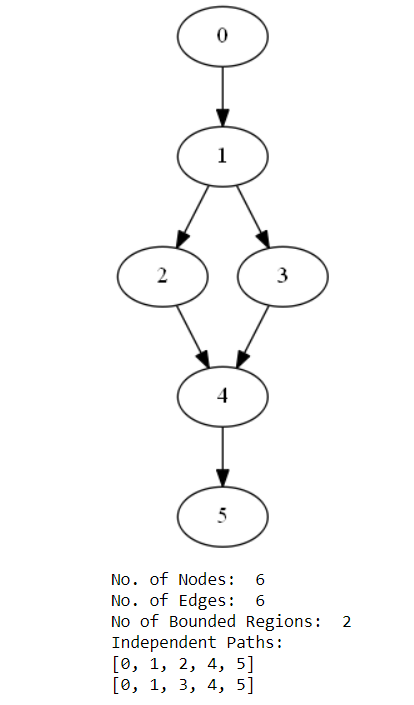
\includegraphics[height=400pt]{1a1}}
\end{center}
\pagebreak
ii) With loop\\
\begin{lstlisting}
for i in range(1,5):
	if i % 2 == 0:
		print("Even Number")
	else:
		print("Odd Number")
\end{lstlisting}
\begin{flushleft}
\textbf{CFG Program:}
\end{flushleft}
\begin{lstlisting}
import pydot
import os
from IPython.display import Image, display
from collections import defaultdict

class Graph: 

    def __init__(self, vertices):  
        self.V = vertices 
        self.graph = defaultdict(list) 

    def addEdge(self, u, v): 
        self.graph[u].append(v) 

    def printAllPathsUtil(self, u, d, visited, path): 

        visited[u]= True
        path.append(u) 

        if u == d: 
            print(path) 
        else: 
            for i in self.graph[u]: 
                if visited[i]== False: 
                    self.printAllPathsUtil(i, d, visited, path) 
        path.pop() 
        visited[u]= False


    def printAllPaths(self, s, d): 

        visited =[False]*(self.V) 
        path = [] 
        self.printAllPathsUtil(s, d, visited, path)

G1 = pydot.Dot(graph_type="digraph")
nodes = [0,1,2,3,4,5,6]
edges = [(0,1),(1,2),(2,3),(2,4),(3,5),(4,5),(5,1),(5,6)]
g1 = Graph(len(nodes))

for i in nodes:
    x = pydot.Node(i)
    G1.add_node(x)
for i in edges:
    x = pydot.Edge(i[0],i[1])
    G1.add_edge(x)
    g1.addEdge(i[0],i[1])

im = Image(G1.create_png())
display(im)

print("No. of Nodes: " , len(nodes))
print("No. of Edges: " , len(edges))
print("No of Bounded Regions: " , (len(edges) - len(nodes) + 2))
print("Independent Paths: ")
g.printAllPaths(nodes[0], nodes[-1])
\end{lstlisting}
\begin{flushleft}
\pagebreak
\textbf{Output:}
\end{flushleft}
\begin{center}
  \makebox[\textwidth]{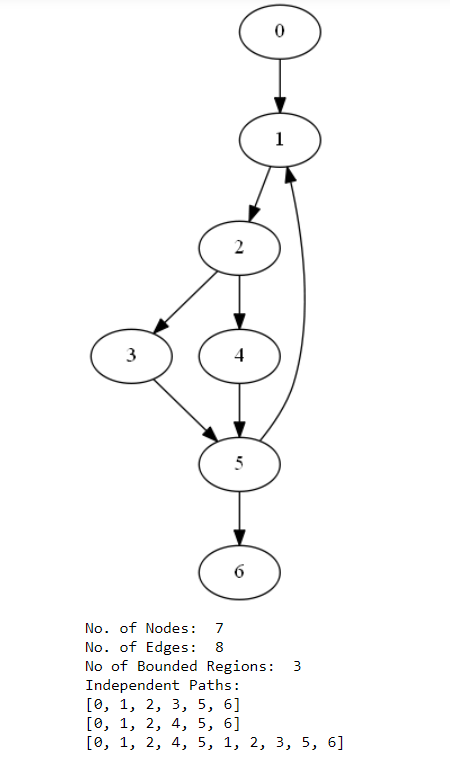
\includegraphics[height=400pt]{1a2}}
\end{center}
\begin{large}
\pagebreak
\textbf{Set 2: Entity-Relationship / Extended Entity Relationship Diagram (ER/EER)}
\end{large}
\begin{flushleft}
\textbf{\emph{A.} NIT Durgapur wants to automate the Student Registration System and seek for intranet based solution. The Candidates  need  to  register  for  some  specific  semester  may  go  online  with  the  system  and  providethe necessary data (roll no., name, department, course, semester and last semester grade point etc.) as input data. The system must able check the input data entered by student from the pre-existing student database and then automatically generate the registration slip for the specific semester as student copy. The system also  will  maintain  a  log  of  the  students  already  registered  and  it  will  restrict  any  duplicate  registration. System Administrator can view and generate report of the list of registered students and list of unregistered students. Draw Suitable ER/EER Diagram.\\}
\end{flushleft}
\textbf{Solution:}\\
Student Registration System entities and their attributes:\\
    $\textbf{1. Student Entity:} \underline{roll\_no}, full\_name, email, course\_id, dept\_id, semester\\
    \textbf{2. Course Entity:} \underline{course\_id}, course\_name, dept\_id\\
    \textbf{3. Department Entity:} \underline{dept\_id}, dept\_name, hod\\
    \textbf{4. Academics Entity:} \underline{roll\_no}, sem\_marks, current\_sem\_reg\_flag\\
    \textbf{5. System administrator Entity:} \underline{user\_id}, pwd, admin\_name\\
    \textbf{6. Reports Entity:} \underline{sr\_no}, roll\_no, reg\_flag\\
    \textbf{7. Registration Entity:} \underline{reg\_id}, roll\_no, trans\_id\\
    \textbf{8. Fees Entity :} \underline{trans\_id}, trans\_date$\\
\textbf{Assumptions:}\\
• It is assumed that this Registration System is prepared for NIT Durgapur students and only those students who had taken admission and already submitted the fees of current semester, can go online to generate the registration slip of that semester as Student’s Copy.\\
• System Administrator can view or modify the student or registration database if needed.\\
• No fee is charged by the System from the students to access their accounts for registration.\\
• The student and registration database are confidential and is NOT available to be used by anyone except the system administrator.\\
• Initially, the student will access the Registration System, provide his/her details like name, roll number, department name, birthdate, course, semester etc., to register for the current semester and then this data will be received by the Registration System to compare it with Student and Registration Database. If the student had not registered previously, then he/she will get registered and the Student Copy of registration will be generated.\\
\begin{center}
  \makebox[\textwidth]{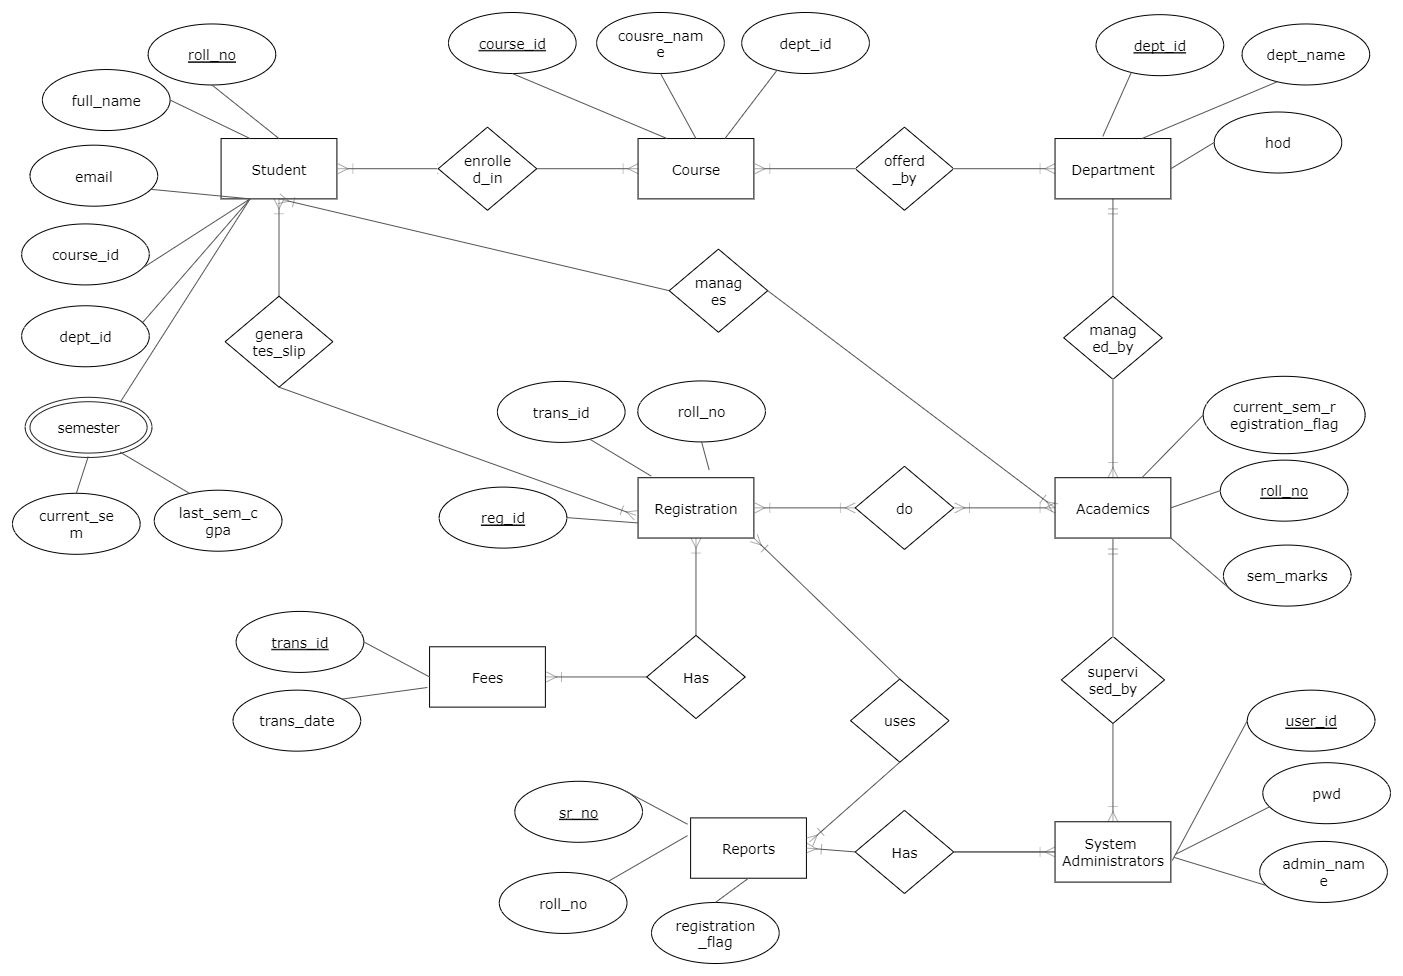
\includegraphics[width=600pt,height=500pt]{2a1}}
\end{center}
\begin{center}
\emph{Figure 1} Student Registration System ER Diagram
\end{center}
\begin{flushleft}
\pagebreak
\textbf{\emph{B.} XYZ Bank is a facilitator for public banking system with many branches in different region. They would like to automate the banking Processing System. The bank facilitates deposit, withdrawal and fixed deposit system from its saving accounts. Customer may have joint account as well as many account in any branch of the bank. Withdrawal or deposit can be done from any branch of the bank. The bank also has facility of ATM. On any transaction, the system will able to maintain the transaction record in some log. Using which, system  administrator  can  generate  report  for  account  wise  transaction  per  day. Draw  Suitable  ER/EER Diagram.}
\end{flushleft}
\textbf{Solution: }\\
Bank Processing System entities and their attributes:\\
    $\textbf{1.) Branch Entity:} \underline{branch\_id}, branch\_name, branch\_address, branch\_manager\\
    \textbf{2.) Customer Entity:} \underline{cust\_id}, cust\_name, aadhar\_no, mobile, dob, cust\_add\\
    \textbf{3.) Accounts Entity:} \underline{acc\_no}, cust\_id, branch\_id, acc\_bal, acc\_type\\
    \textbf{4.) ATM Entity:} \underline{atm\_id}, atm\_add, trans\_id\\
    \textbf{5.) Transaction Entity:} \underline{trans\_id}, trans\_date, trans\_amt, trans\_type, from\_acc\\
    \textbf{6.)  System Administrators Entity:} \underline{user\_id}, pwd, admin\_name$
\textbf{Assumptions:}\\
• It is assumed that the customers who have Bank Account and Bank Passbook as proof or have ATM card with valid Pin Code will only use this Bank Processing System.\\
• It is also assumed that the customer database such as name, addresses and other details, already exists in the Processing System.\\
• No fee will be charged by the Processing System from the customers to process deposit or withdrawal from his/her account.\\
• The resources and database of the Processing System are highly confidential and are NOT available to be used by anyone except system administrator.\\
• The documentation shows the relationship among the Branch, Customer and their account in that branch, including cash transaction slips, ATMs, customer databases and transaction logs.\\
• Initially the customer will go the bank branch or ATM to deposit or withdraw the cash and then get his/her transaction slip. Also, the system administrator can be able to generate daily transaction logs.\\
\begin{center}
  \makebox[\textwidth]{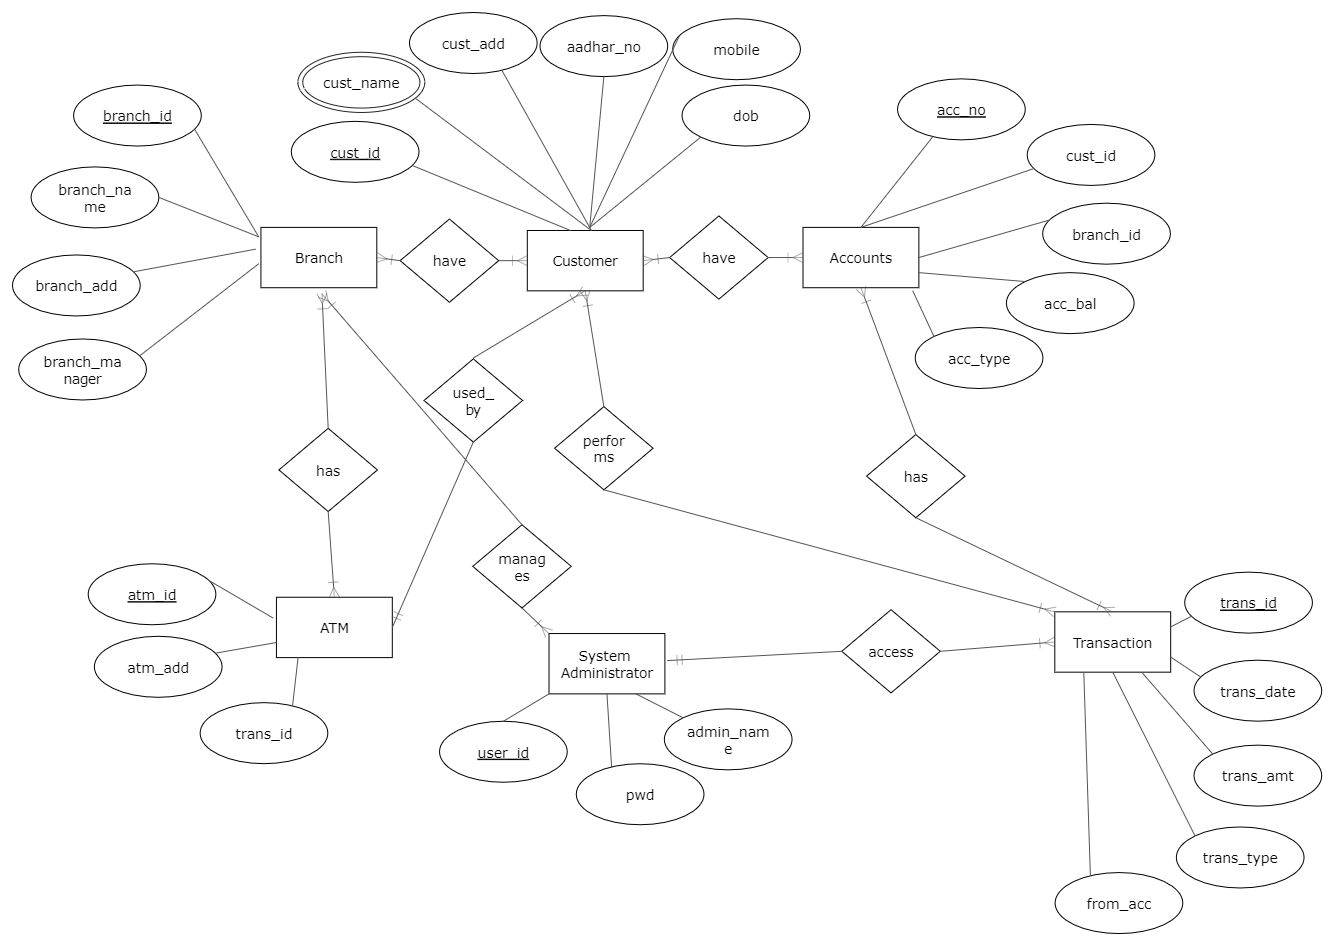
\includegraphics[width=600pt,height=500pt]{2b1}}
\end{center}
\begin{center}
\emph{Figure 2} Bank Processing System ER Diagram
\end{center}
\begin{large}
\pagebreak
\textbf{Set 3: Unified Modelling Language (UML)}
\end{large}
\begin{flushleft}
\textbf{\emph{A.}Consider Automated Teller Machine (ATM) based withdrawal of cash. For  any account it will check if Minimum balance is available for withdrawal and can disburse cash maximum of INR 10,000/-. ATM can accept debit cards of pre-specified banks (more than one). On every transaction, the machine will generate a  report.  Draw  Use  Case  diagram,  Class  diagram,  Object  Diagram,  Sequence  Diagram  for  the  above activities.}
\end{flushleft}
\begin{center}
  \makebox[\textwidth]{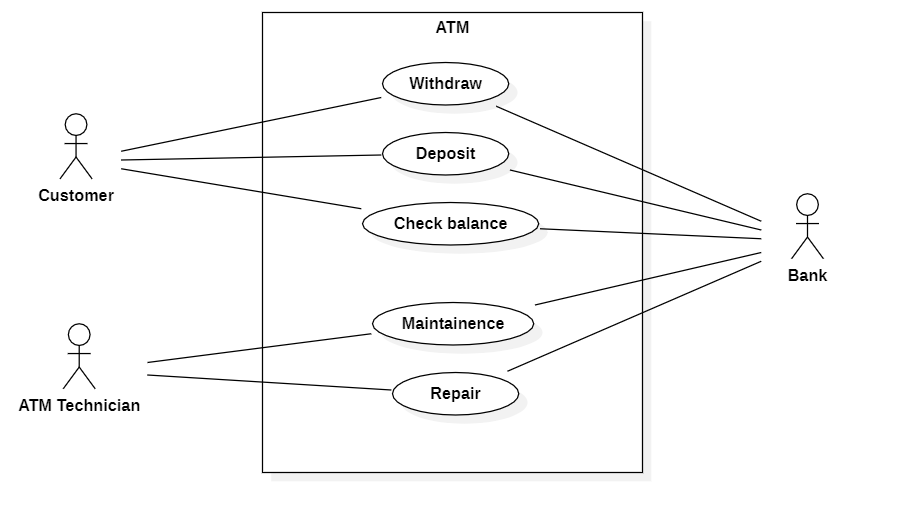
\includegraphics[width=600pt,height=450pt]{3a1}}
\end{center}
\begin{center}
\emph{Figure 3} Use Case Diagram for ATM
\end{center}
\begin{center}
  \makebox[\textwidth]{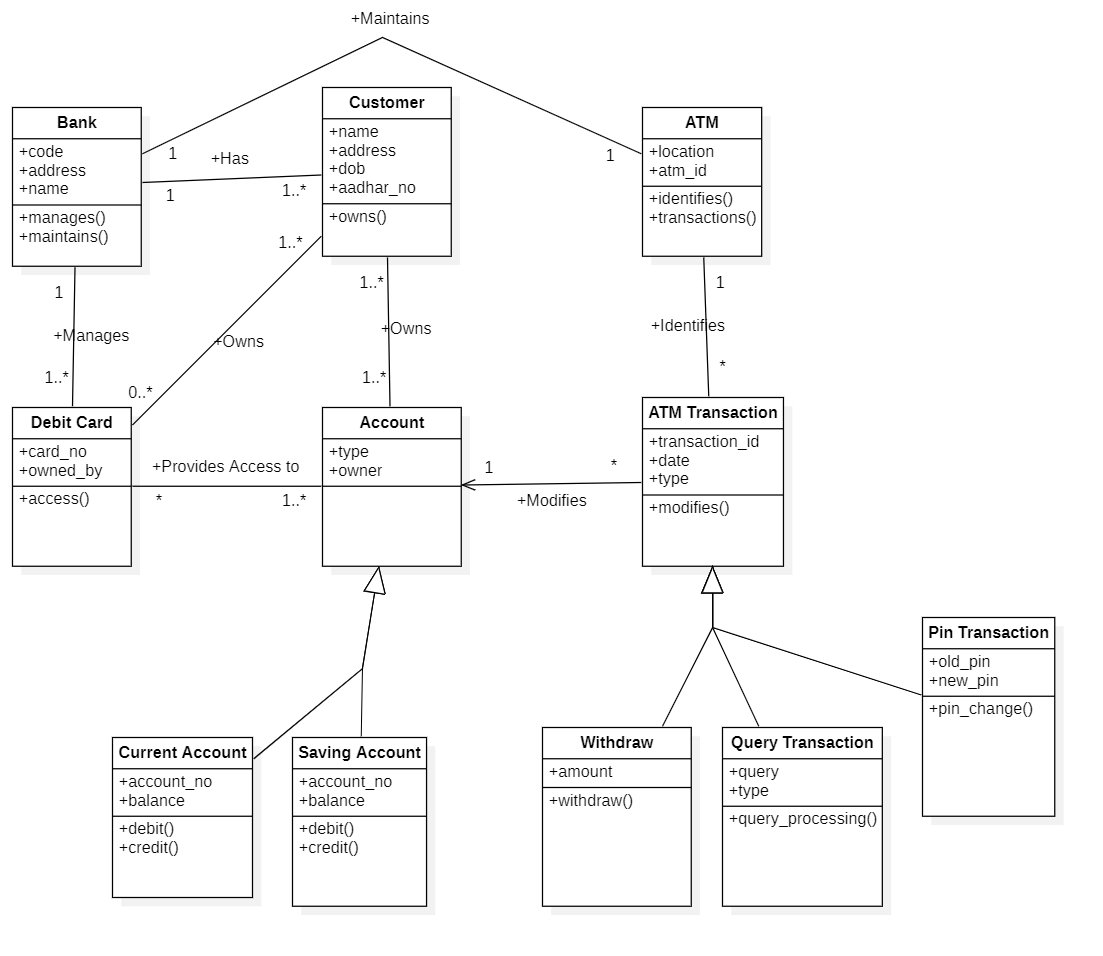
\includegraphics[width=600pt,height=500pt]{3a2}}
\end{center}
\begin{center}
\emph{Figure 4} Class diagram for ATM
\end{center}
\begin{center}
  \makebox[\textwidth]{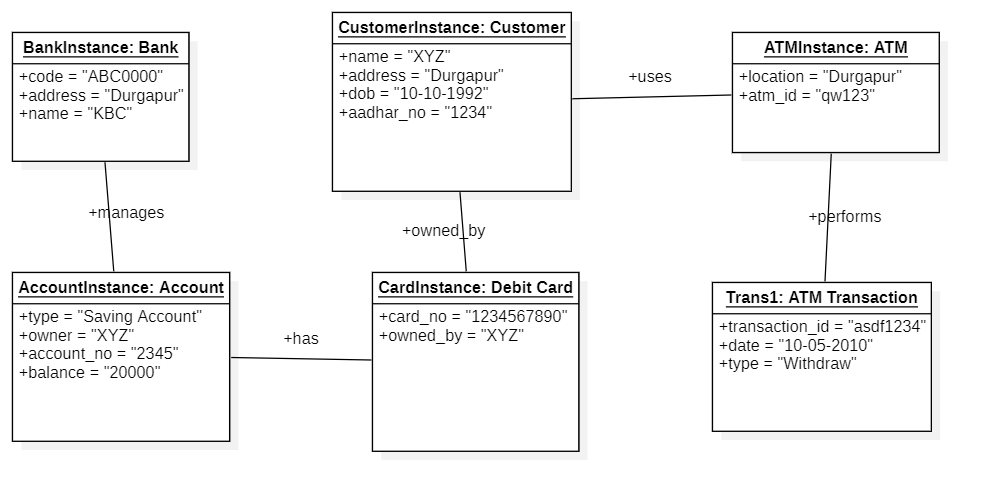
\includegraphics[width=600pt,height=500pt]{3a3}}
\end{center}
\begin{center}
\emph{Figure 5} Object Diagram for ATM
\end{center}
\begin{center}
  \makebox[\textwidth]{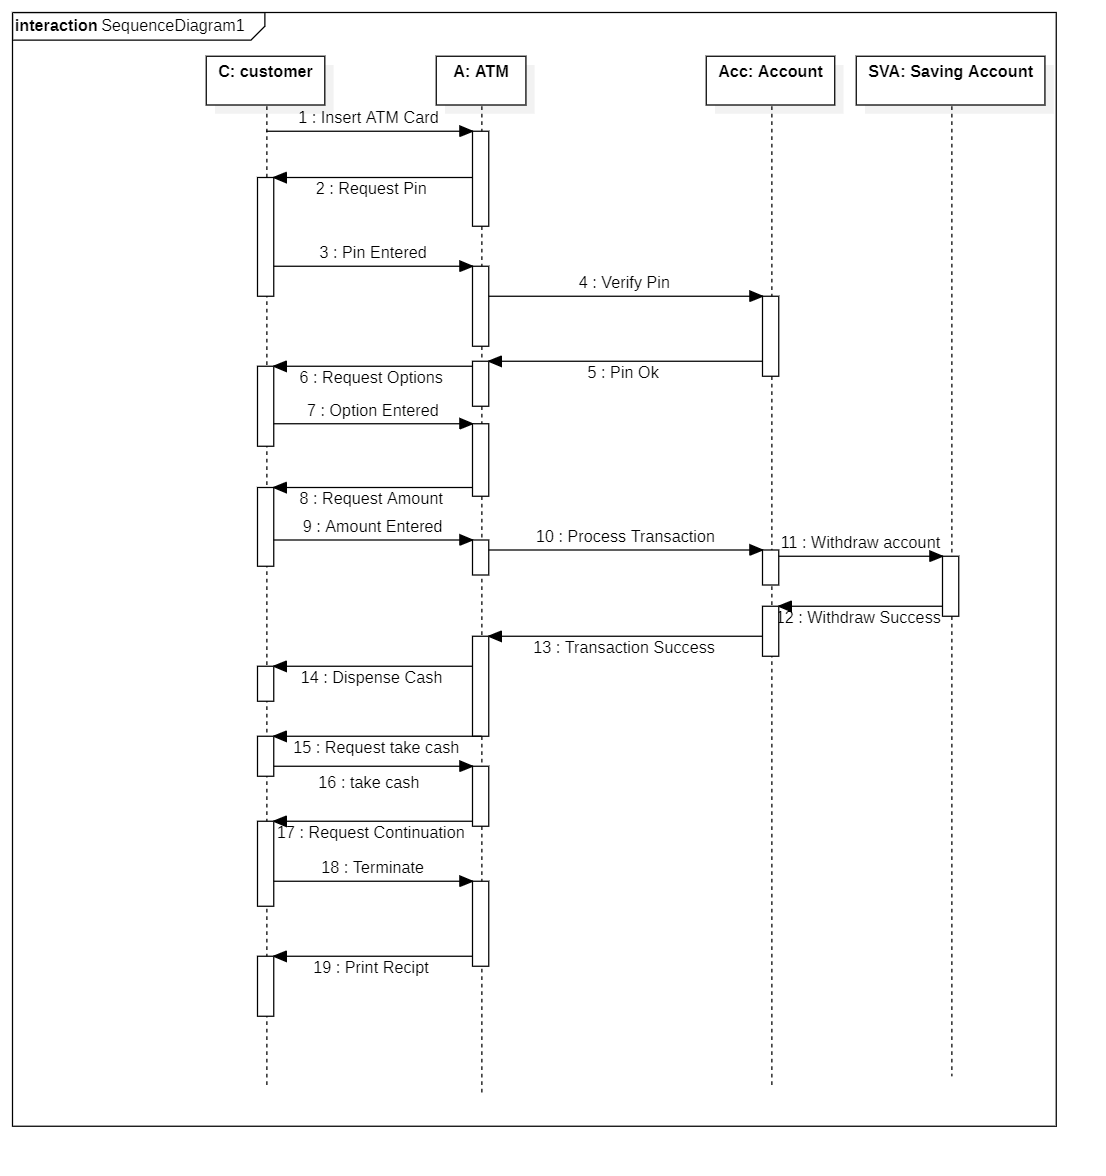
\includegraphics[width=600pt,height=600pt]{3a4}}
\end{center}
\begin{center}
\emph{Figure 6} Sequence Diagram for ATM
\end{center}
\begin{flushleft}
\textbf{\emph{B.} A Clinic Centre would like to implement a system to maintain the Patient’s Visit Records. The system will keep  and  update  the  information  related  to  Registration,  Out  Patient  Department  visits,  related  Doctor Information  and  Medical  history  (Patient  Wise).All  records  will  be  maintained  with  respect  to  the Registration Number of Patients. On Registration, each Patient is normally attached with a medical advisor (Role of Doctor) for necessary guidance. One advisor may guide several Patients at any point of time. Draw Use Case diagram, Class diagram, Object Diagram, Sequence Diagram for the above activities.}
\end{flushleft}
\begin{center}
  \makebox[\textwidth]{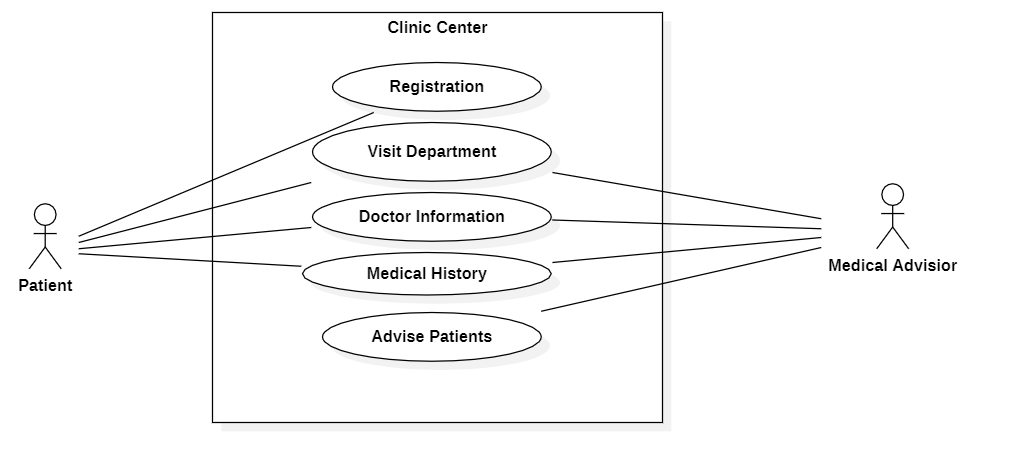
\includegraphics[width=600pt,height=450pt]{3b1}}
\end{center}
\begin{center}
\emph{Figure 7} Use case Diagram for Clinic Center
\end{center}
\begin{center}
  \makebox[\textwidth]{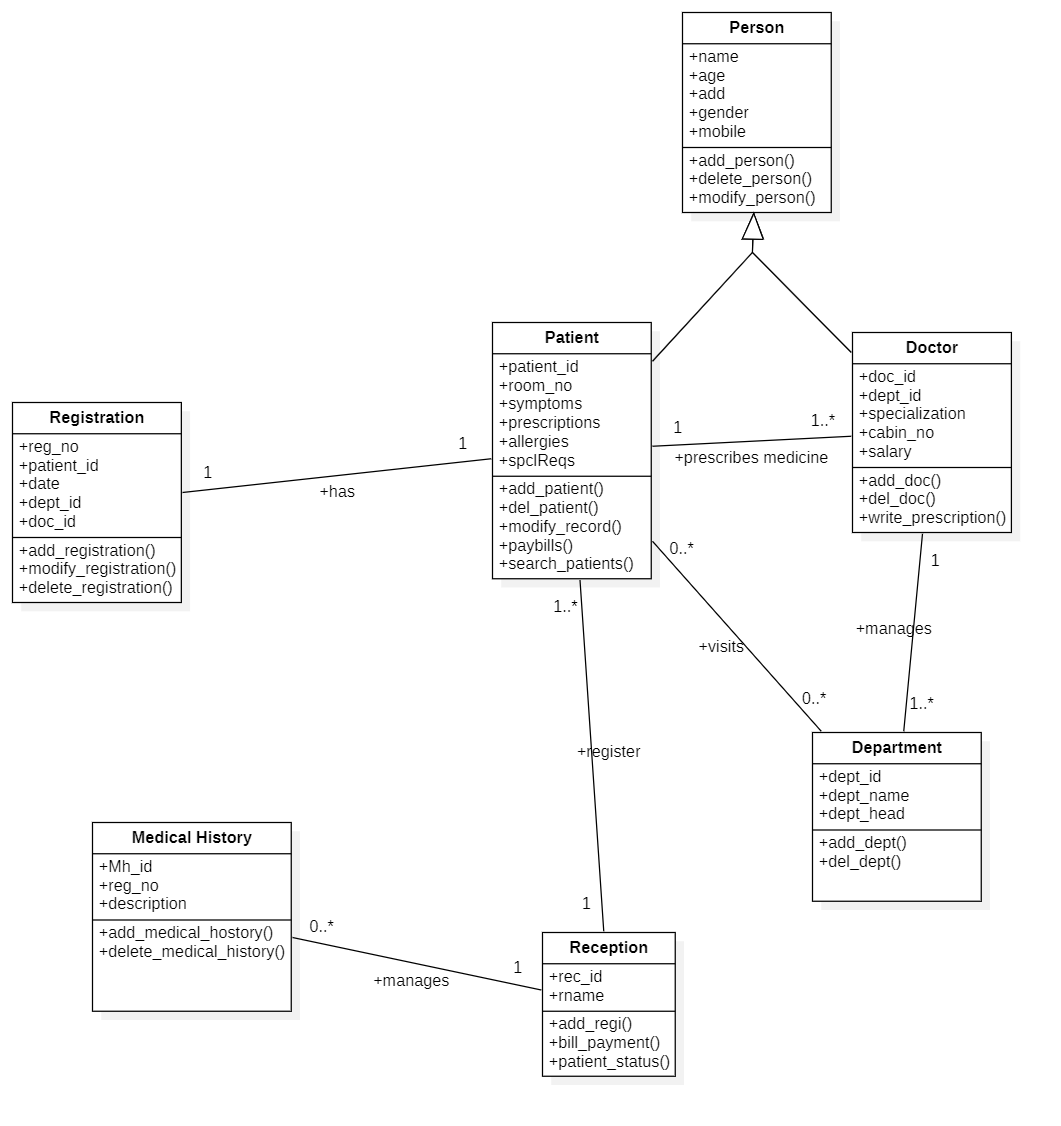
\includegraphics[width=600pt,height=500pt]{3b2}}
\end{center}
\begin{center}
\emph{Figure 8} Class Diagram for Clinic Center
\end{center}
\begin{center}
  \makebox[\textwidth]{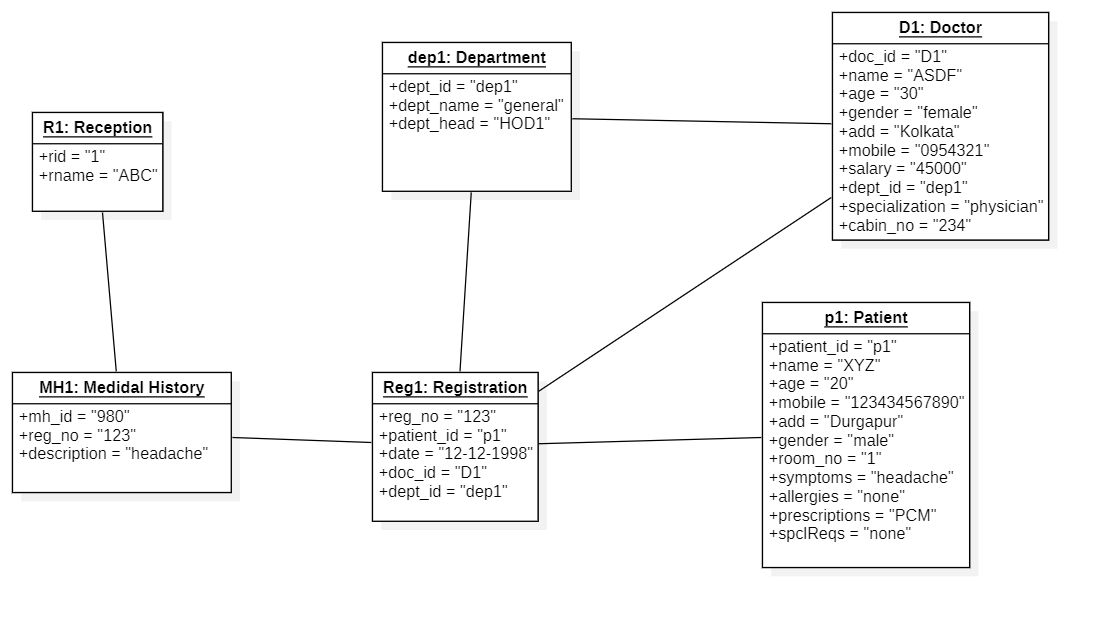
\includegraphics[width=600pt,height=500pt]{3b3}}
\end{center}
\begin{center}
\emph{Figure 9} Object diagram for Clinic Center
\end{center}
\begin{center}
  \makebox[\textwidth]{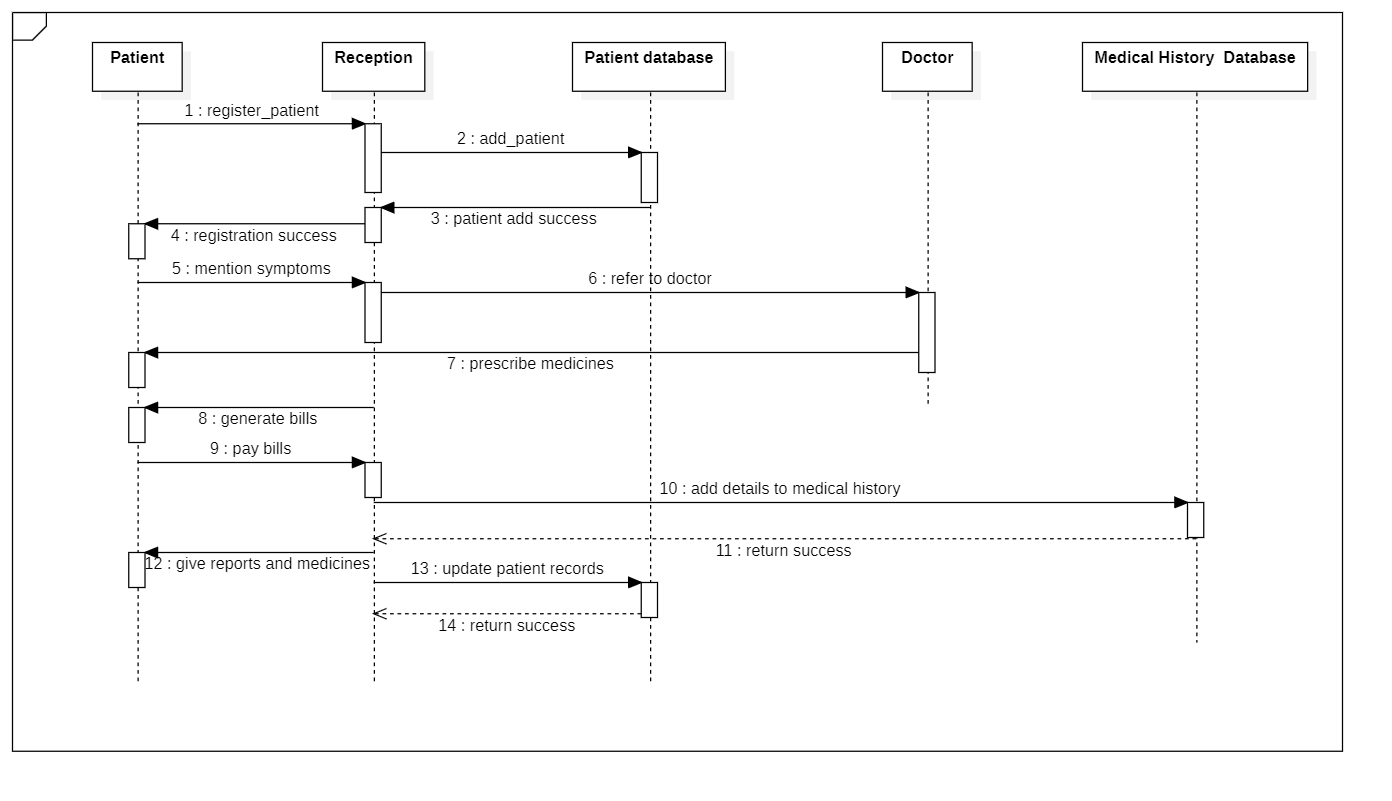
\includegraphics[width=600pt,height=600pt]{3b4}}
\end{center}
\begin{center}
\emph{Figure 10} Sequence Diagram for Clinic Center
\end{center}
\end{document}
